\documentclass{standalone}
\usepackage[margin=1in]{geometry}
\usepackage[hang,small,bf]{caption}
\usepackage{tikz}
\usepackage{braket}
\usetikzlibrary{backgrounds,shadows.blur,fit,decorations.pathreplacing,shapes}

\begin{document}
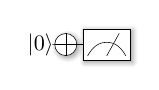
\begin{tikzpicture}[scale=0.8, transform shape]

\tikzstyle{basicshadow}=[blur shadow={shadow blur steps=8, shadow xshift=0.7pt, shadow yshift=-0.7pt, shadow scale=1.02}]\tikzstyle{basic}=[draw,fill=white,basicshadow]
\tikzstyle{operator}=[basic,minimum size=1.5em]
\tikzstyle{phase}=[fill=black,shape=circle,minimum size=0.1cm,inner sep=0pt,outer sep=0pt,draw=black]
\tikzstyle{none}=[inner sep=0pt,outer sep=-.5pt,minimum height=0.5cm+1pt]
\tikzstyle{measure}=[operator,inner sep=0pt,minimum height=0.5cm, minimum width=0.75cm]
\tikzstyle{xstyle}=[circle,basic,minimum height=0.35cm,minimum width=0.35cm,inner sep=-1pt,very thin]
\tikzset{
shadowed/.style={preaction={transform canvas={shift={(0.5pt,-0.5pt)}}, draw=gray, opacity=0.4}},
}
\tikzstyle{swapstyle}=[inner sep=-1pt, outer sep=-1pt, minimum width=0pt]
\tikzstyle{edgestyle}=[very thin]

\node[none] (line0_gate0) at (0.1,-0) {$\Ket{0}$};
\node[xstyle] (line0_gate1) at (0.5,-0) {};
\draw[edgestyle] (line0_gate1.north)--(line0_gate1.south);
\draw[edgestyle] (line0_gate1.west)--(line0_gate1.east);
\draw (line0_gate0) edge[edgestyle] (line0_gate1);
\node[measure,edgestyle] (line0_gate2) at (1.15,-0) {};
\draw[edgestyle] ([yshift=-0.18cm,xshift=0.07500000000000001cm]line0_gate2.west) to [out=60,in=180] ([yshift=0.035cm]line0_gate2.center) to [out=0, in=120] ([yshift=-0.18cm,xshift=-0.07500000000000001cm]line0_gate2.east);
\draw[edgestyle] ([yshift=-0.18cm]line0_gate2.center) to ([yshift=-0.07500000000000001cm,xshift=-0.18cm]line0_gate2.north east);
\draw (line0_gate1) edge[edgestyle] (line0_gate2);

\end{tikzpicture}
\end{document}
